%**********************************************************************
% Base layout + including standard packages
%**********************************************************************
\documentclass[a4paper,12pt]{report}

% allows direct input of special chars
\usepackage[utf8]{inputenc}  

%**********************************************************************
% YOUR SETTINGS - START
%**********************************************************************

% About your study degree programme
\def \study{ITM} % possible options: 
          % ITM ... for BA in Software Design and Cloud Computing (vz vollzeit / ft full-time)
          % SWD ... for BA in Software Design and Cloud Computing (bb berufsbegleitend / pt part-time)
          % MSD ... for BA in Mobile Software Development
          % IRM ... for MA in IT-Recht and Management
          % IMS ... for MA in IT and Mobile Security

% More about you and your thesis:
\def \title{Optimierung von Datenströmen zwischen Frontend und Backend: 
	gRPC im Vergleich zu REST und GraphQL}
\def \subtitle{}
\def \yourName{Michael Mühlberger}
\def \yourIdentifier{<1700000017>} % Used for Seminar Work / Projektarbeit ONLY
\def \yourPlace{Kapfenberg}
\def \submissionDate{Juni 2025}  % month year. e.g. June 2017
\def \yourAdvisor{DI MA Michael Ulm}  


\def \thisDocumentIsA{Thesis} % possible options:
                    % Thesis  .... for Master's Thesis   / Masterarbeit
                    % Thesis  .... for Bachelor's Thesis / Bachelorarbeit
                    % Seminar .... for Seminar Work      / Seminararbeit
                    % Project .... for Project Work      / Projektarbeit

% ITM/SWD/IRM: you could possibly write in German.
\def \yourLanguage{german} % possible options:
                 % english
                 % german

%**********************************************************************
% YOUR SETTINGS - END
%**********************************************************************



% LaTeX preamble = include a lot of packages, configure latex settings
%**********************************************************************
% Various LaTeX packages
%**********************************************************************


% programming (branching) logic
\usepackage{ifthen}

% you might need some mathematical expressions:
\usepackage{amsmath}

% with package babel we allow to use language english and german
\usepackage[english,german]{babel}


% permits to set space between lines
\usepackage{setspace}  	

% ensure proper appearance of all fonts in pdf:
\usepackage[T1]{fontenc}

% lmodern after T1 fontenc (_may_ be required)
% lmodern = Latin Modern fonts
%\usepackage{lmodern}  	

%\usepackage{times} -- obsolete; use:
% Times as default text font, maths support
\usepackage{mathptmx}  	
% provides bold font (required for syntax highlighting in listings)
\usepackage{courier}  	

% enables table cells to span multiple rows
\usepackage{multirow}  
% paragraphs: no indentation at beginning, but spacing between  
\usepackage{parskip}  	

% for figures
\usepackage[pdftex]{graphicx}
% implicit file name extensions for embedded figures 
% so we do not need to specify the extension on inclusion
\DeclareGraphicsExtensions{.pdf,.jpg,.png}

% for flexible tables (e.g. auto resizing to page width) 
%     e.g.: { | l | l | X | }
\usepackage{tabularx}

%**********************************************************************
% Including non-standard packages
%**********************************************************************

% abbreviations are written in full length on first time usage
% e.g. with \acro{UX}{User Experience} 
%    \ac{UX} first time: User Experience (UX)
%    \ac{UX} later:      UX 
\usepackage{acronym}

% http://en.wikibooks.org/wiki/LaTeX/Colors
\usepackage[usenames,dvipsnames,table]{xcolor}
% we define a few custom colors  
\definecolor{gray20}{gray}{0.8}
\definecolor{gray5}{gray}{0.95}
\definecolor{olivegreen30}{RGB}{155,187,89}  

\usepackage{alltt}

% for code snippets, embedded as "listings"
\usepackage{listings}
% we set a few defaults below with \lstset:

  
% the page layout (geometry), 
% as defined by FH guidelines (2.3 Formale Gestaltung):
\usepackage[top=3cm, 
            bottom=3cm, 
            left=3.5cm, 
            right=3cm]
           {geometry}

% superscript st first,
%             nd second
%             rd third
%             th fourth,...
\usepackage[super]{nth}     % 1st, 2nd, 3rd,...

%\usepackage{paralist}   	% inline lists
%\usepackage{mdwlist}
\usepackage{enumitem}

% e.g. for "floating" listings (no fixed anchor in text)
\usepackage{float}     
\floatstyle{plain}
\restylefloat{figure}
% e.g. to show two (floating) images side-by-side
\usepackage{subfig}

% add copyright information to figures
\usepackage{copyrightbox} 



% symbols such as \texttimes and \texteuro
\usepackage{textcomp}  
% math. symbols from the American Mathematical Society  
%\usepackage{amssymb}  	


% chapter heading styles
% see 3.2 The Chapter Lenny at
%         https://ctan.org/pkg/fncychap
\usepackage[Lenny]{fncychap}  

% for \enquote, \textquote, \blockquote...
\usepackage[autostyle]{csquotes}       

% how to create simple helper commands (LaTeX "macros"):
% e.g. red-coloured text when using ...
%      \TODO{Do not forget to add further references}
\newcommand{\TODO}[1]
{
{\textcolor{red}{[TODO: #1]}}
}


% Create/style more complex new commands:
% e.g. \chapquote{Phone home!}{by E.T.}
% BEGIN: chapquote
\newcommand{\chapquote}[2]  
{%
\begin{quote}
\emph{%
``#1''%
}%
\begin{flushright}
{\scriptsize \sffamily [#2]}%
\end{flushright}
\end{quote}
}
% END: chapquote



% Biblatex = bibliography for LaTeX
% ---------------------------------------------------------------------
% context sensitive quotation; recommended for usage with Biblatex
\usepackage{csquotes}  	
% Note: \date, \origdate, \eventdate, and \urldate 
%       require "yyyy-mm-dd" format,
%       so "dd" or "mm-dd" may be omitted
\usepackage[backend=biber,
            urldate=long,  	        % [Feb. 8, 2027]
                                    %                  default: short 
                                    %                  e.g. 08/15/2010
            style=authoryear-icomp, % Harvard citation style    
                                    %   author, year: ... (cf. Batina et al., 2012, p. 317) 
                                    %   icomp: compact & ibidem: ... see (cf. ibid., p. 317) 
                                    %   see: https://tug.ctan.org/info/biblatex-cheatsheet/biblatex-cheatsheet.pdf 
            backref,                % if you like (cit. on p. 2)
            % sorting=nty, 	        % this is default: sort by name,
                                    %                  title, year
            % sortlocale=de_DE,     % set according to your needs
            natbib=true,  	        % use "natbib"-compatible citation
                                    %                  commands
                                    % do _not_ use package natbib!
            maxbibnames=1000,  	    % show all authors in the 
                                    %                  bibliography
            % ibidpage=true,        % this is default for ibid / 
                                    %                  ebd ("ebenda")                        
            giveninits=true,        % E. B. White instead of Elwyn Brooks White
            uniquename=minyearfull, % Reference Authors with same lastname without initials 
                                    % (otherwise set to  "init")
]{biblatex}

% using & instead of "and"
\renewcommand*\finalnamedelim{\addspace\&\space}

% We enforce strict Harvard style: 
% The URL date default is "(Visited on ...);" => so:
%     BibTeX entries such as:
%      url = {http://...},
%      urldate = {2015-05},
%      urldate = {2015},
%      urldate = {2015-05-17},
%     shall be printed as
%      Available from: <http://...> [May 17, 2015]
\DeclareFieldFormat{urldate}{\mkbibbrackets{#1}}
\ifthenelse{\equal{\yourLanguage}{german}}{
  % for language = german: 
  % [online ] https://dl.acm.com/paper3.pdf [17. Mai 2015]
  \DeclareFieldFormat{url}{[online]\space \url{#1}}
}{ % else: 
   % default language = english
   % Available from: https://dl.acm.com/paper3.pdf [May 17, 2015]
  \DeclareFieldFormat{url}{Available\space from\addcolon\space \url{#1}}
}



% ---------------------------------------------------------------------
% !!
% hyperref should be last package loaded
% !! 
\usepackage[  	              
    pdftitle={\title},
    pdfsubject={\thisDocumentIsA},
    pdfauthor={\yourName},
    pdftex,  	              % driver
    breaklinks,  	          % permits line breaks for long links
    bookmarks,  	          % create Adobe bookmarks
    bookmarksnumbered,        % ... and include section numbers
    linktocpage,  	          % the page number (not the text) is link on TOC
    colorlinks,  	          % 
    linkcolor=black,          % normal internal links;
    anchorcolor=black,        % don't make scientific papers too colourful
    citecolor=black,
    urlcolor=blue,  	      % blue is quite common for urls
    pdfstartview={Fit},       % "Fit" fits the page to the window
    pdfpagemode=UseOutlines,  % open bookmarks in Acrobat
    plainpages=false,         % avoids duplicate page number problem
    pdfpagelabels,
  ]{hyperref}

% we break our rules from above and specify another package AFTER hyperref
% allow to specify multiple refs at once, using \Cref{ }
% e.g. \Cref{lst:hello,lst:closure}
\usepackage{cleveref}


%**********************************************************************
% A hack to allow the urls to break on some more characters
%**********************************************************************

% Uncomment, if you want to break URLs at . @ / ! _ | % ; > .... 
%\def\UrlBigBreaks{\do\.\do\@\do\\\do\/\do\!\do\_\do\|\do\%\do\;\do\>\do\]%
% \do\)\do\,\do\?\do\'\do\+\do\=\do\#\do\:\do@url@hyp}

% Uncomment, if you want to break URLs at 123456789 
%\def\UrlBreaks{\do\1\do\2\do\3\do\4\do\5\do\6\do\7\do\8\do\9}

% Uncomment, if you want to break URLS at abcde....xyz and ABCDE....XYZ  
%\def\UrlBreaks{\do\a\do\b\do\c\do\d\do\e\do\f\do\g\do\h\do\i\do\j\do\k\do\l%
%               \do\m\do\n\do\o\do\p\do\q\do\r\do\s\do\t\do\u\do\v\do\w\do\x%
%               \do\y\do\z%
%               \do\A\do\B\do\C\do\D\do\E\do\F\do\G\do\H\do\I\do\J\do\K\do\L%
%               \do\M\do\N\do\O\do\P\do\Q\do\R\do\S\do\T\do\U\do\V\do\W\do\X%
%               \do\Y\do\Z%
%}

% To break URLs in the bibliography
% "bib url lc penalty" will add a breakpoint after all lowercase letters. 
\setcounter{biburllcpenalty}{7000} 
% "bib url uc penalty" will add a breakpoint after all lowercase letters.
\setcounter{biburlucpenalty}{8000} 



%**********************************************************************
% Layout adjustments
%**********************************************************************

% page layout (header/footer and page numbers) 
\pagestyle{headings} % options:
         % headings
         % fancy
         % empty

% Optimise headers / footers
%   when printing the first page of a (numbered) chapter 
%   suppress the page number (on center bottom)
\newcommand{\chapterstart}{\thispagestyle{empty}}
%   when printing the first page of the bibliography
%   suppress the page number (on center bottom)
\AtBeginBibliography{\thispagestyle{empty}}

         
% settings for structure and numbering 
%  we allow three levels within text:  1.2.1 
\setcounter{secnumdepth}{3}
%  but we show two levels in TOC: 1.2
\setcounter{tocdepth}{1}



% command "\chapterend" to close a chapter 
% (flush, i.e. print remaining figures and tables)
\newcommand{\chapterend}
           {\newpage{
              \pagestyle{empty}
               \cleardoublepage
             }
           }

% footnotes: no indent, hanging
\usepackage[hang,flushmargin]{footmisc}

% new environment for smaller paragraphs
% e.g. \begin{spar}A paragraph with some indentation.\end{spar}
\newenvironment{spar}
{\begingroup \leftskip 0.7cm \rightskip\leftskip}
{\par \endgroup}
% ^^^ must be set here (or use empty line)


%**********************************************************************
% LaTeX macros and commands to style the ISBN and color code listings
%**********************************************************************



% Bibliography: distinguish between cited and non-cited entries
%               so it is possible to show non-cited entries as 
%               Further Readings
\DeclareBibliographyCategory{cited}
\AtEveryCitekey{\addtocategory{cited}{\thefield{entrykey}}}

% Bibliography: we create links for given ISBN
\DeclareFieldFormat{isbn}{\isbn{#1}}
\newcommand{\isbn}[1]
{%
{%
\ifpdf
{\small ISBN}
\href{https://isbnsearch.org/isbn/#1}{#1}%
\else
{\small ISBN}
#1%
\fi
}%
}


% You might define support for further programming languages
% when using listings
\usepackage{color}
\definecolor{lightgray}{rgb}{.9,.9,.9}
\definecolor{darkgray}{rgb}{.4,.4,.4}
\definecolor{purple}{rgb}{0.65, 0.12, 0.82}
\lstdefinelanguage{JavaScript}{
  keywords={break, case, catch, continue, debugger, default, delete, do, else, false, finally, for, function, if, in, instanceof, new, null, return, switch, this, throw, true, try, typeof, var, void, while, with},
  morecomment=[l]{//},
  morecomment=[s]{/*}{*/},
  morestring=[b]',
  morestring=[b]",
  ndkeywords={class, export, boolean, throw, implements, import, this},
  keywordstyle=\color{blue}\bfseries,
  ndkeywordstyle=\color{darkgray}\bfseries,
  identifierstyle=\color{black},
  commentstyle=\color{purple}\ttfamily,
  stringstyle=\color{red}\ttfamily,
  sensitive=true
}

\lstset{numbers=left, 
        basicstyle=\footnotesize\ttfamily,  
        showstringspaces=false,
        % numbers=none           % disable line numbering
        captionpos=b,            % caption at bottom
        breaklines=false, 
        numbersep=5pt,           % space for numbers
        caption={Listing subtitles could and should contain whole sentences
                 describing the important aspect of the listing.}, 
        float=tbhp,             % float listing to top/bottom/here/page
        language=JavaScript,     % Python Ruby SQL ksh erlang ...
        frame=single,
        breaklines=true,         % break long source code lines, add arrow
        postbreak=\mbox{\textcolor{red}{$\hookrightarrow$}\space},
        basewidth={0.55em}, 
}



%**********************************************************************
% Special hyphenation rules
%**********************************************************************

\hyphenation{JOANNEUM}  	% extend to your needs

%**********************************************************************
% Different settings for ITM / SWD / IRM / IMS
%**********************************************************************


% ITM = Internettechnik
% SWD-CC(vz) was formerly called : "Internettechnik"
% ------------------------
\ifthenelse{\equal{\study}{ITM}}{
  \def \theStudyProgramme {Software Design and Cloud Computing}
  \def \isBachelorThesis {}
}
%\fi

% SWD = Software Design
% SWD-CC(pt) was formerly called : "Software Design"
% ------------------------
\ifthenelse{\equal{\study}{SWD}}{
  \def \theStudyProgramme {Software Design and Cloud Computing}
  \def \isBachelorThesis {}
}

% MSD = Mobile Software Development
% ------------------------
\ifthenelse{\equal{\study}{MSD}}{
  \def \theStudyProgramme {Mobile Software Development}
  \def \isBachelorThesis {}
}


% IRM = IT-Recht & Management
% -------------------------------
\ifthenelse{\equal{\study}{IRM}}{
  \def \theStudyProgramme {IT-Recht \& Management}
  \def \isMasterThesis {}
}

% IMS = IT & Mobile Security
% ------------------------------
\ifthenelse{\equal{\study}{IMS}}{
  \def \theStudyProgramme {IT \& Mobile Security}
  \def \isMasterThesis {}
}


 

% Add one (or multiple) file(s) with bibliography entries:
%   here "thesis.bib" i.e. pdflatex sets \jobname to 'thesis'
%   the name specified when running pdflatex
%   \addbibresource{thesis.bib}
\addbibresource{\jobname.bib}





\begin{document}
%**********************************************************************
% Structure of thesis: inclusion of chapters
%**********************************************************************
\ifthenelse{\equal{\yourLanguage}{german}}{
  \selectlanguage{german}
}{ % else: default language = english
  \selectlanguage{english}
}




\ifthenelse{\equal{\thisDocumentIsA}{Thesis}}{  
  % a title page is included for BA/MA Thesis only
  %**********************************************************************
% right side, if two-sided
\chapterend

\begin{titlepage}

\begin{center}
% scale image according to the actual logo you use
% official JPG ist way too large, so [height=2.5cm] is required
% official EPS, converted to PDF:

\includegraphics[height=1cm]
                {images/logo_FHJ_100mm_cmyk.pdf}
\hfill

% the actual title
\mbox{}\vfill

  \large

  {\huge\bf \title \par}
  \subtitle
  \vspace{2.0cm}
  
\ifdefined\isMasterThesis % MA

  \ifthenelse{\equal{\yourLanguage}{german}}{ % German Version 

   {\bf Masterarbeit}\\
    zur Erlangung des akademischen Grades\\
   
    \ifthenelse{\equal{\study}{IRM}}{ % IRM Master of Arts
  
      {\bf Master of Arts in Business (MA)}\\
      eingereicht am\\
      Fachhochschul-Studiengang {\bf \theStudyProgramme \\}
  
    }{  % else: IMS = Master of Science
      
      {\bf Master of Science in Engineering (MSc)}\\
      eingereicht am\\
      Fachhochschul-Studiengang {\bf \theStudyProgramme \\}
      
   }

  }{ % English Version 

    {\bf Master's Thesis}\\
    submitted in conformity with the requirements for the degree of\\
   
    \ifthenelse{\equal{\study}{IRM}}{ % IRM Master of Arts
  
      {\bf Master of Arts in Business (MA)}\\
      Master's degree programme {\bf \theStudyProgramme \\}
  
    }{  % else: IMS = Master of Science
      
      {\bf Master of Science in Engineering (MSc)}\\
      Master's degree programme {\bf \theStudyProgramme \\}
      
   }

  } 
\else % BA
  
  \ifthenelse{\equal{\yourLanguage}{german}}{ % German Version 
  
  {\bf Bachelorarbeit}\\
  zur Erlangung des akademischen Grades\\
  {\bf Bachelor of Science in Engineering (BSc)}\\
  
  eingereicht am\\
  Fachhochschul-Studiengang {\bf \theStudyProgramme \\}

  }{ % English Version 
  
  {\bf Bachelor's Thesis}\\
  submitted in conformity with the requirements for the degree of\\
  {\bf Bachelor of Science in Engineering (BSc)}\\
  Bachelor's degree programme {\bf \theStudyProgramme \\}

  }

\fi
  
  \vspace{0.5cm}

 FH JOANNEUM  (University of Applied Sciences), Kapfenberg

  \vspace{1.5cm}

  \mbox{}

  \ifthenelse{\equal{\yourLanguage}{german}}{ % German Version

  {\bf Betreuer/in: \yourAdvisor\\
   % Zweit-/Firmenbetreuer/in: <Vorname Zuname; Firmenname>

  Eingereicht von: \yourName
  }
  
  
  }{ % English Version 

  {\bf Supervisor: \yourAdvisor\\ 
  % second supervisor: <firstname lastname; company>

  Submitted by: \yourName
  }
  
  }

  \vspace{1.5cm}

   \submissionDate
  
  \vspace{1.5cm}
% \TODO{Specify the title, sub title, place, date, study, language, 
	% your name, and advisor in the main \emph{thesis.tex} file.\\
	% Finally, remove all \emph{TODOs} within your \LaTeX source code.}


\end{center}

\vfill\mbox{}


\end{titlepage}



%**********************************************************************

}{ 
  \ifthenelse{\equal{\thisDocumentIsA}{Seminar}}{ 
    % Seminar Work (se)
    %**********************************************************************
% right side, if two-sided
\chapterend

\begin{titlepage}

\begin{center}
% scale image according to the actual logo you use
% official JPG ist way too large, so [height=2.5cm] is required
% official EPS, converted to PDF:

\includegraphics[height=1cm]
                {images/logo_FHJ_100mm_cmyk.pdf}
\hfill

% the actual title
\mbox{}\vfill

  \large

  {\huge\bf \title \par}
  \subtitle
  \vspace{2.0cm}
  
  \ifthenelse{\equal{\yourLanguage}{german}}{ % German Version 

   {\bf Seminararbeit}
   

  }{ % English Version 

    {\bf Seminar Work}
  } 

  
  \vspace{0.5cm}

 FH JOANNEUM  (University of Applied Sciences), Kapfenberg

  \vspace{1.5cm}

  \mbox{}

  \ifthenelse{\equal{\yourLanguage}{german}}{ % German Version

  {\bf Betreuer/in: \yourAdvisor\\
   % Zweit-/Firmenbetreuer/in: <Vorname Zuname; Firmenname>

  Eingereicht von: \yourName\\
  Personenkennzahl: \yourIdentifier}
  
  
  }{ % English Version 

  {\bf Supervisor: \yourAdvisor\\ 
  % second supervisor: <firstname lastname; company>

  Submitted by: \yourName\\
  Personal identifier: \yourIdentifier}
  
  }

  \vspace{1.5cm}

   \submissionDate
  
  \vspace{1.5cm}
  \TODO{Specify the title, sub title, place, date, study, language, your name, advisor and your id in the preamble in file thesis.tex.}

\end{center}

\vfill\mbox{}


\end{titlepage}



%**********************************************************************

  }{
    % Project Work (pw)
    %**********************************************************************
% right side, if two-sided
\chapterend

\begin{titlepage}

\begin{center}
% scale image according to the actual logo you use
% official JPG ist way too large, so [height=2.5cm] is required
% official EPS, converted to PDF:

\includegraphics[height=1cm]
                {images/logo_FHJ_100mm_cmyk.pdf}
\hfill

% the actual title
\mbox{}\vfill

  \large

  {\huge\bf \title \par}
  \subtitle
  \vspace{2.0cm}
  
  \ifthenelse{\equal{\yourLanguage}{german}}{ % German Version 

   {\bf Projektarbeit}
   

  }{ % English Version 

    {\bf Project Work}
  } 

  
  \vspace{0.5cm}

 FH JOANNEUM  (University of Applied Sciences), Kapfenberg

  \vspace{1.5cm}

  \mbox{}

  \ifthenelse{\equal{\yourLanguage}{german}}{ % German Version

  {\bf Betreuer/in: \yourAdvisor\\
   % Zweit-/Firmenbetreuer/in: <Vorname Zuname; Firmenname>

  Eingereicht von: \yourName\\
  Personenkennzahl: \yourIdentifier}
  
  
  }{ % English Version 

  {\bf Supervisor: \yourAdvisor\\ 
  % second supervisor: <firstname lastname; company>

  Submitted by: \yourName\\
  Personal identifier: \yourIdentifier}
  
  }

  \vspace{1.5cm}

   \submissionDate
  
  \vspace{1.5cm}
  \TODO{Specify the title, sub title, place, date, study, language, your name, advisor and your id in the preamble in file thesis.tex.}

\end{center}

\vfill\mbox{}


\end{titlepage}



%**********************************************************************

  }
}


% Anmerkung: 
%    NUR gesperrte Arbeiten werden gedruckt und benötigen eine 
%    Eidesstattliche Erklärung / Signed Declaration
%\include{chapters/02_declaration} 


%**********************************************************************

%---------------------------------------------------
% NOTE:
% An English version of the abstract is always required 
% (even for German BA/MAs).
%---------------------------------------------------

% right side/flush
\chapterend

\begin{titlepage}

\begin{otherlanguage}{english} 

\begin{abstract} % Abstract
\label{abstract_english}
While gRPC is a well-known and used API approach for service-to-service communication in microservice architecture with high performance requirements, gRPC-Web is still less common on the web. The performance benefits of gRPC, are primarily due to binary Protocol Buffers (Protobuf) serialization format and HTTP/2 multiplexing.
Since most browsers do not support the full set of HTTP/2 features, gRPC-Web cannot fully leverage these advantages. Therefore, REST and GraphQL still remain the dominant web API approaches for web clients.
The goal of the Bachelos thesis is to evaluate how gRPC-Web performs compared to REST and GraphQL with respect to latency, efficiency and resource usage and to identify scenarios in which using gRPC-Web for frontend-backend communication is suitable.
The methodology combines a theoredical analysis with an experimental evaluation using a custom-built prototype. The prototype implements several services that cover typical web payloads (e.g.text or media data) and supports tests both in a browser-based web client and a microservice scenario. The measurement series includes single and parallel requests, cross-browser comparison and a contrast between browser-based frontend-backend communication an service-service communication in the microservice scenario.
Measurements show that, in the browser context, gRPC-Web is not a viable performance-oriented replacement for REST or GraphQL. Especially for large media payloads, REST outperforms both gRPC-Web and GraphQL. Although the theoretical analysis showed that Protocol Buffers more efficient than JSON, these advantages were not measurable. This is due to the limited availability of HTTP/2 features in browsers and the additional proxy/translation layer which is required by gRPC-Web. Another disadvantage compared to REST and GraphQL is, that gRPC-Web is harder to learn and has has less documentation, tools and community support.
Overall gRPC still remains the best option for service-to-service communication in microservice architectures, particularly under high request rates and high performance requirements, the use of gRPC-Web in browsers is just useful, when an existing gRPC backend needs to be exposed to browsers. Improved browser support for HTTP/2 and HTTP/3 could change this assessment in the future.


\end{abstract}

\end{otherlanguage}


\end{titlepage}


%---------------------------------------------------
% NOTE:
% A German version of the abstract "Zusammenfassung"
% is always required.
%---------------------------------------------------

\begin{titlepage}

\begin{otherlanguage}{german}

\begin{abstract}  % Zusammenfassung
\label{abstract_german}

Während gRPC bereits als etablierter Standard für die Service-zu-Service in Microservice-Architekturen gilt, ist gRPC-Web im Web-Kontext weniger verbreitet. Die Leistungsvorteile von gRPC basieren insbesondere auf der binären Protobuf-Serialisierung und HTTP/2-Multiplexing. Da Browser wichtige HTTP/2-Features nur eingeschränkt unterstützen, kann gRPC-Web diese Vorteile nicht vollständig nutzen. Im Browserumfeld dominieren daher weiterhin REST und GraphQL als etablierte Web-API-Ansätze.
Diese Bachelorarbeit befasst sich mit den Fragen, wie sich gRPC-Web im Vergleich zu den etablierten Web-Technologien REST und GraphQL auf Latenz, Effizienz und Ressourcennutzung in der Frontend-Backend-Kommunikation zwischen einem Web-Client und einem Web-Server auswirkt und unter welchen Bedingungen der Einsatz von gRPC für die Frontend-Backend-Kommunikation sinnvoll ist.
Für die Beantwortung dieser Fragen wird ein kombinierter methodischer Ansatz gewählt: eine theoretischen Analyse und eine experimentelle Evaluation anhand eines eigens entwickelten Prototyps, der die End-zu-End Latenz aus Sicht des Frontend Clients misst. 
Der Prototyp implementiert mehrere Services, die typische Web-Payloads (wie Text- und Mediendaten) abdecken, und Tests sowohl im Browser (Web-Client) als auch in einem Microservice-Szenario (Konsolen-Client). Basierend darauf werden Messreihen mit Einzel- und Parallelenabfragen durchgeführt, verschiedene Browserumbebungen verglichen und die Frontend–Backend-Kommunikation im Browser der Service-zu-Service-Kommunikation im Microservice-Szenario gegenübergestellt.
Die Messungen deuten darauf hin, dass gRPC-Web im Browserumfeld nicht mit den etablierten Web-API-Ansätzen REST und GraphQL konkurrenzfähig ist. Die in der Theorie erwarteten Performanceverbesserungen durch Protobuf konnten durch die Prototypen im Browser nicht bestätigt werden. Grund dafür sind die fehlenden HTTP/2-Features im Browser und der zusätzliche Übersetzungsschritt von gRPC zu gRPC-Web. Zusätzlich ist der Erlernbarkeit von gRPC-Web  im Vergleich zu etablierten Technologien wie REST komplexer und es stehen weniger Dokumentation, Tools und Community-Ressourcen zur Verfügung. Vor allem bei großen Binärdaten erwies sich REST im Browser als robuster.
Insgesamt empfiehlt sich gRPC weiterhin vor allem für Service-zu-Service Szenarien mit hoher Requestfrequenz während eine Implementierung von gRPC-Web nur dann sinnvoll ist, wenn bereits ein gRPC-basiertes Backend besteht. Bei verbesserter Browser-Unterstützung für HTTP/2 oder HTTP/3 könnte sich dies künftig ändern. 


\end{abstract}

\end{otherlanguage}

\end{titlepage}

%**********************************************************************


% optional:
%%**********************************************************************

% Optional: add acknowledgement
\chapterend

\begin{titlepage}

\begin{center}\large\bf

\ifthenelse{\equal{\yourLanguage}{german}}{ % German Version
 Danksagung 
}{ % English Version
 Acknowledgement 
}
\end{center}
Your text here\ldots
\TODO{Optionally, you might say thank you or give credits to someone.}

\end{titlepage}


%**********************************************************************
 

\chapterend

\pagenumbering{roman}  	% roman page numbers for title pages


\tableofcontents            % TOC = Table-of-Contents

% OPTIONALLY, adding single entries (LoF, LoT, LoL) to TOC: 

% Adding entry LoF "List of Figures / Abbildungsverzeichnis" to TOC
\clearpage
\addcontentsline{toc}{chapter}{\listfigurename} 
\listoffigures

% Adding entry LoT "List of Tables / Tabellenverzeichnis" to TOC
\clearpage
\addcontentsline{toc}{chapter}{\listtablename}
\listoftables 

% Adding entry LoL "List of Code Snippets" to TOC
% \clearpage
% \addcontentsline{toc}{chapter}{List of Code Snippets}
% \lstlistoflistings

\chapterend





\pagenumbering{arabic}  % ... for ordinary chapters
\onehalfspacing



% remove this, when starting to write your thesis:
%%%%%%%%%%%%%%%%%%%%%%%%%%%%%%%%%%%%%%%%%%%%%%%%%%%%%%%%%%%%%%%%%%%%%%%%%%%%%
\chapter{Writing a Thesis Using \LaTeX{} }
\label{chap:info_REMOVE_ME}
%%%%%%%%%%%%%%%%%%%%%%%%%%%%%%%%%%%%%%%%%%%%%%%%%%%%%%%%%%%%%%%%%%%%%%%%%%%%%
\chapterstart

\chapquote{Research is formalised test curiosity. It is poking and prying with
a purpose.}
          {Zora Neale Hurston}

Each chapter should start with a short explanation what is inside the
upcoming chapter and why it has been included (at this position) in your
work: This template shall provide some considerations, text examples and
formatting hints for your Bachelor's or Master's thesis in \LaTeX{}.


\section{Hints on Scientific Writing}

Some recommendations on writing an abstract and about including references to
related work.

\subsection{How to Write an Abstract}

Learn from others and read many papers\footnote{For examples, read the
abstract of paper \url{https://arxiv.org/abs/1609.03677}.} related to your
work. Finally, you might ensure that your abstract contains:

	\begin{itemize}
		\item English \& German Version (250 – 350 words each)
		\item Background / motivation / problem statement
		\item Methods / procedure / approach
		\item Results / findings / product
		\item Conclusion and implications
	\end{itemize}

It is easier to write the Abstract when the rest of your paper is finished.

\subsection{Research Resources}


For literature research use e.g.
\citetitle{acm:diglibrary}~\parencite{acm:diglibrary} or
\citetitle{ieee:xplore}~\parencite{ieee:xplore}.
You might start your search within the scientific databases
\url{http://dl.acm.org/} or \url{http://ieeexplore.ieee.org/}.
Full-text PDF download is available from within the FH JOANNEUM network.


\subsection{Citation Styles}

% Ensure, that the concepts of
%  o parenthetical citation
%  o narrative citation
%  o direct quotation
%  are clear to you
Harvard citation style is implemented in this template. For information about
a topic like RFID paraphrased in your own
words~\parencite[cf.][p. 317]{Batina:2011}, \parencites{Chen:2021, Chen:2023} do not forget to use \emph{cf.}
and -- if available the relevant page number(s) -- along with parenthetical
cite \verb+\parencite+. Direct quotations would not need the \emph{cf.}.
% Recently, many publications do not strictly require the cf. all the time.
% It is recommended to use cf., but cf. is not strictly required anymore.
The abbreviation \emph{cf.} is short for Latin \emph{confer} meaning compare.
The abbreviation \emph{p.} is short for \emph{page}, and \emph{pp.} is short for \emph{pages}.
If you need to use the title of a reference, for example the RFID Authentication
Protocol by \citetitle{Fernandez-Mir:2011} you might use \verb+\citetitle+.
For references without parentheses such as -- find more in \cite{Li:2008}
-- just use \verb+\cite+ or, if year should be in parentheses,
\textcite{Batina:2011} \verb+\textcite+.

\begin{spar}
  Note the use of \emph{ibid}. \emph{Ibid} is short for Latin \emph{ibidem}
  meaning in the same place. In German \emph{ebd} or \emph{ebenda} is used.
  \emph{Ibid} is used for referencing (several pages of) the same resource
  subsequently. For example,
  see \citep[cf.][p. 317]{Batina:2011} and \citep[cf.][pp. 321-–323]{Batina:2011}
  \citep[cf.][p. 399]{Batina:2011}.
\end{spar}

You might cite URLs, e.g. about (tools for checking)
Accessibility~\parencite[cf.][]{Google:2017a,Google:2016a}, as online
resources with a date of your last visit.


% TODO Add selected examples of resources and citations:
% URLs
% Books
% Conference Papers
% White/Yellow Papers
% Specifications
% Internal (company) papers
% ...
% arxiv (not peer-revied)


\subsection{Bibliography Entries}

Compile your resources you want to cite in a file with so called bibliography
entries \emph{bib entries}.
Readers must be able to trace back and verify each and every source.
Make sure, reades can find the given resources quick and easily.

The required information to provide might differ between the kind of resources.
Every entry needs information on author(s), title, and year.
For books you need to add the publisher information and the ISBN.
For research papers (from scientific databases such as IEEE or ACM)
one need to add the conference title, location and the \ac{DOI}.
For articles in journals it is suggested, that the series entry is available,
as for \cite{Chen:2023}.
For the DOI and \ac{ISBN} numbers, links are automatically generated by \LaTeX,
hence no full link (\ac{URL}) must be specified.

\subsection{Scientific Writing Resources}

% Write intro for items ending with a ":" colon

Selected resources about scientific working:
\begin{itemize}
  \item \emph{\citetitle{Zobel:2004}}: \ldots elements of good writing
      -- clarity, simplicity, accuracy, and organization \ldots by
      \cite{Zobel:2004}.

  \item \emph{\citetitle{Shaw:2002} }: \ldots e.g. find out ways of validating your findings, your results \ldots by \cite{Shaw:2002}.


  \item \emph{\citetitle{Yin:2013}}: \ldots offers comprehensive coverage of
      the design and use of the case study method as a valid research tool
      \ldots by \cite{Yin:2013}.

  \item \emph{\citetitle{Strunk:2000}}: \ldots first edition about 1935;
      includes a list of valuable recommendations: be clear, do not overwrite
      \ldots by \cite{Strunk:2000}.

  \item \emph{\citetitle{Field:2003}}: \ldots Planning an Experiment,
      Experimental Designs, Descriptive Statistics, Inferential Statistics
      \ldots Answering the Question 'So What?' \ldots by \cite{Field:2003}.

  \item \emph{\citetitle{Booth:2008}}: \ldots What Is Research? Creating a
      Relationship with Your Reader: Your Role, Finding a Good Research
      Problem \ldots by \cite{Booth:2008}.

  \item \emph{\citetitle{Alley:1998}}: \ldots your writing is the principle
      way in which people learn about your work. When you communicate well,
      you receive credit for your \ldots by \cite{Alley:1998}.

  \item \emph{\citetitle{Eco:2010}}: \ldots Warum muss man eine
      wissenschaftliche Abschlussarbeit schreiben und was ist sie? \ldots by
      \cite{Eco:2010}.

  \item \emph{\citetitle{Wisconsin:2004}}: \ldots you will find many
      instructional materials we've developed for our Writing Center
      teaching: Planning and Writing Research Papers, Creating an Argument,
      \ldots by \cite{Wisconsin:2004}.

\end{itemize}

Better take a look at those references \emph{before} starting to write
your thesis.


\section{\LaTeX{} Formatting Hints}

Selected \LaTeX{} examples are included to give an impression of how you could add tables, diagrams, or figures to your text. Use \emph{bullet lists} and \emph{emphasised} text and \emph{named paragraphs} sparsely.

% example for a named paragraph
\paragraph{Background.} In the section on the background describe
the prerequisites for your work.

\paragraph{Terms and definitions.}
Technical terms should be explained if necessary. Abbreviations are
summarised at the end of the thesis in Chapter~\ref{chap:acronyms}
``\nameref{chap:acronyms}''. The abbreviations are defined in advance
using \verb+\acro{}{}+. Within the text \verb+\ac{}+ is used. For
example, \verb+\ac{ABI}+ and \verb+\ac{MITM}+ occur in text
as \ac{ABI} and \ac{MITM}. If \verb+\ac{ABI}+ is used again, only
the acronym \ac{ABI} is printed (as hyperlink though).

\paragraph{Visual elements.}
To support your readers, include visuals such as diagrams and other graphics
(see Figure~\ref{fig:engine}). Note the short title used for the list of
figures.




\begin{figure}[tp]
  \centering
  \copyrightbox[r]{
  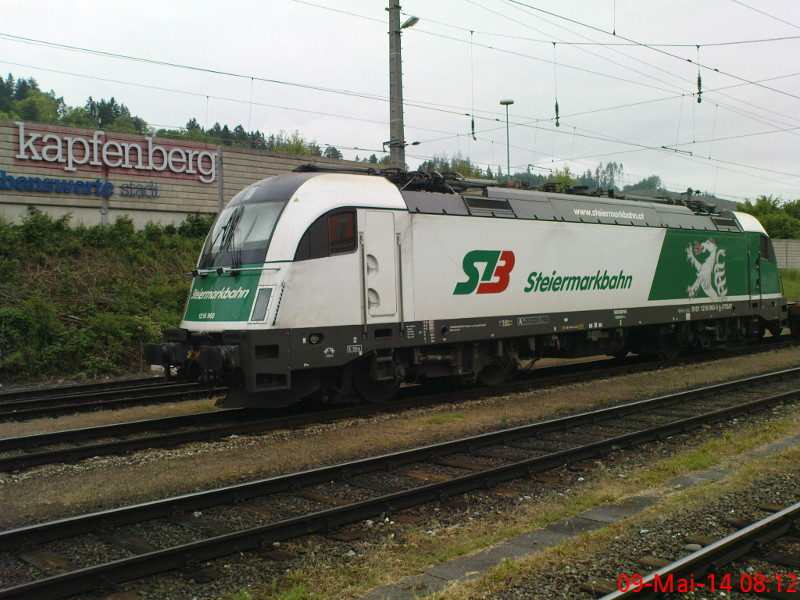
\includegraphics[keepaspectratio,
                   width=0.95\textwidth]
                  {images/engine}
  }{\tiny \copyright~Diethard Ohrt}
  % The short caption should be capitalised
  % The full caption should hold a full sentence including a full stop (.)
  \caption[Logo at the Train Engine]
          {Note the logo attached to the train
           engine spotted in Kapfenberg main station.}
  \label{fig:engine}
\end{figure}

Code listings require the \verb+listings+ package which, in turn,
requires some settings. This is, because the defaults do not fit all
purposes; see command \verb+\lstset{}+ in preamble of this template.
Additionally, the package \textit{courier} should be used because the
defaults do not provide for proper syntax highlighting\footnote{
Find the full list of supported programming languages at
\url{https://www.overleaf.com/learn/latex/Code_listing}.
}. Very small code snippets \lstinline$ func main(){...}$ can be marked with \verb+\lstinline{}+ in the text.



In order to see what's possible when formatting tables -- here are two fancy
tables, see Table~\ref{tab:olive} and Table~\ref{tab:grey} which show
demo data. Preferable, use  \verb+tabularx+, because the parameter \emph{X}
allows to define columns of dynamic size. Online table generators\footnote{Online table generator \url{https://www.tablesgenerator.com}.} can create the \LaTeX source for you.

\begin{center}
  \begin{table}[tp]
    \begin{tabularx}{\textwidth}{|l|l|p{1,8cm}|X|}\hline
      \rowcolor{olivegreen30}
      \textcolor{white}{\textbf{Version}}
         &\textcolor{white}{\textbf{Description}}
           &  \textcolor{white}{\textbf{Author(s)}}
             &\textcolor{white}{\textbf{Date}}\\
      \hline
      1.0
        & Initial
          & Ohrt
            & July 15, 2014\\
      \hline
      1.1
        & Filled section ``Open Issues''
          & Ohrt
            & July 16, 2014\\
      \hline
      1.2
        & Added section ``Restrictions''
          & Ohrt
            & September 15, 2014\\
      \hline
      1.3
        & Dynamic fields for ``BA'' and ``MA''
          & J.F.
            & September 15, 2018\\
      \hline
      1.4
        & Restructuring many sections
          & J.F.
            & November 127, 2019\\
      \hline
      \end{tabularx}
    \caption[Fancy Table]{Olive green heading used for this fancy table.}
    \label{tab:olive}
  \end{table}
\end{center}

 \begin{center}
  \begin{table}[tbp]
    \begin{tabular}{ l | l }
      \rowcolor{gray20}\textbf{Error}
        & \textbf{Solution} \\
      \rowcolor{gray5}Java.lang.OutOfMemoryError: PermGen space
        & -XX:MaxPermSize=1024M \\
      \rowcolor{gray5}\textit{(32-/64-bit issue)}
        & \\
      \rowcolor{gray20}Error occurred during initialization of VM \textit{or}
        & increase or remove -Xms value \\
      \rowcolor{gray20}Could not reserve enough space for object heap
        & e.g.\ -Xms128m -Xmx512m \\
      \rowcolor{gray20}
        & \small{(Eclipse default:}\\
      \rowcolor{gray20}
        & \small{-Xms40m -Xmx512m)} \\
    \end{tabular}
    % The short caption should be capitalised
    % The full caption should hold a full sentence.
    \caption[Simple Grey Table]
            {A more or less simple grey table. Better try to put tables and
             figures at \textit{top}[t] or at the \textit{bottom}[b] of a
             page. With \textit{page}[p] you can put them on a separate page.
             Avoid location specifier \textit{here}[h].}
    \label{tab:grey}
  \end{table}
\end{center}


Always reference listings in text, such as Listing~\ref{lst:democlosure}.
Use line numbers to help the reader to find relevant parts within given code.
Referenced listings, tables and figures are written in uppercase first
letter: \emph{L}isting X,  \emph{T}able Y and  \emph{F}igure Z.


\subsection{Prototype}

Find in Listing~\ref{lst:democlosure} an example of the JavaScript closure.
Only selected (relevant) parts of the original source code have been
included. That allows to extract and display parts of working code!







Hints on listings: use environment \verb+samepage+ for not breaking the
listing in multiple parts and not spreading the listing over multiple pages
(see \Cref{lst:democlosure,lst:hello}). Do not forget to make the
listings float with \verb+float=tp+.

% Demo of an inline source code listing
\begin{samepage}
	\begin{lstlisting}[float=tbhp,
	                   caption={[Hello in C] No programming language
	                            for syntax highlighting is specified,
	                            hence the default we specified in
	                            lst, i.e. \emph{C}, is taken.},
	                   label=lst:hello,
	                  ]
void main(int argc, char *argv[])
{
  printf("Hello world!");
}
	\end{lstlisting}
\end{samepage}


\begin{samepage}
  \lstinputlisting[language=JavaScript,
                   float=tp,                % float to the "best" place
                   aboveskip=\floatsep,
                   belowskip=\floatsep,
                   xleftmargin=0cm,         % no extra margins for floats
                   xrightmargin=0cm,        % no extra margins for floats
                   label=lst:democlosure,   % reference to this listing
                   firstline=10,            % include just a few lines
                   lastline=88,             % of the given file
                   caption={[Closure]       % Short Title for LOL
                             Demo implementation of a
                             JavaScript \emph{Closure}.}
                  ]{src/closure.js}         % the file to be included
\end{samepage}

Mathematical expressions are rendered beautifully by \LaTeX. Now enjoy
the first Maxwell equation
\begin{math}
  \text{rot} \vec{H} = \vec{J} + \frac{\partial \vec{D}}{\partial t}
\end{math}.
%
Simple mathematical expressions can be written inline enclosed between
\verb+$+, such as $ax^2+bx+c = 0$. Important equations should stand out and
be put into dedicated \verb+equation+ environment. They get numbered
automatically.
\begin{equation}
  \frac{a^2}{b - c} = 8
\end{equation}


\section{Sentences and Praragraphs}

For better readability, try to structure long text into paragraphs. Insert
a newline between paragraphs. paragraphs should not be too short, they are
expected to contain several sentences.

\section{Red Thread} % Roter Faden

At the end of each chapter you might sum up the contents of the chapter in
a sentence or two. Then you might tell the reader what will be presented in
the upcoming section (to make her/him curious).


\TODO{You have seen how \LaTeX~works; now remove this Chapter.}

\vfill
% next chapter: start at right side, if two-sided; else just flush page
\chapterend
     % LaTeX examples  



% Add chapters as required. For example 

%%%%%%%%%%%%%%%%%%%%%%%%%%%%%%%%%%%%%%%%%%%%%%%%%%%%%%%%%%%%%%%%%%%%%%%%%%%%%
\chapter{Introduction}
\label{chap:intro}
%%%%%%%%%%%%%%%%%%%%%%%%%%%%%%%%%%%%%%%%%%%%%%%%%%%%%%%%%%%%%%%%%%%%%%%%%%%%%
\chapterstart

% Overall problem
%  and why is it relevant 
%  relevant to which target group
% key questions to answer
% your approach, the method (survey, prototype, user tests, ...)
% one/two hypotheses (idea of solution)

Your text here\ldots 
\TODO{Describe the kind of problem at hand? The problem is relevant in which 
context? What does not work well at the moment? 
What do people need? Describe the background, the prerequisites for your 
work. Optionally, add terms and definitions whenever they might not be clear 
to a fellow student. test ~\parencite{Brooks:1975} }

%%%%%%%%%%%%%%%%%%%%%%%%%%%%%%%%%%%%%%%%%%%%%%%%%%%%%%%%%%%%%%%%%%%%%%%%%%%%%
\section{Problem Statement}\label{sec:problem}
%%%%%%%%%%%%%%%%%%%%%%%%%%%%%%%%%%%%%%%%%%%%%%%%%%%%%%%%%%%%%%%%%%%%%%%%%%%%%

Your text here\ldots 
\TODO{What is the overall problem? Give examples. Motivate! Compared to 
existing solutions for the problem at hand, why does someone need a better, 
faster, and somewhat different one?
test }


%%%%%%%%%%%%%%%%%%%%%%%%%%%%%%%%%%%%%%%%%%%%%%%%%%%%%%%%%%%%%%%%%%%%%%%%%%%%%
\section{Research Questions}\label{sec:rq}
%%%%%%%%%%%%%%%%%%%%%%%%%%%%%%%%%%%%%%%%%%%%%%%%%%%%%%%%%%%%%%%%%%%%%%%%%%%%%

Your text here\ldots 
\TODO{Focus on one or two main research questions and detail on them.}

%%%%%%%%%%%%%%%%%%%%%%%%%%%%%%%%%%%%%%%%%%%%%%%%%%%%%%%%%%%%%%%%%%%%%%%%%%%%%
\section{Hypothesis}\label{sec:hypothesis}
%%%%%%%%%%%%%%%%%%%%%%%%%%%%%%%%%%%%%%%%%%%%%%%%%%%%%%%%%%%%%%%%%%%%%%%%%%%%%


Your text here\ldots 
\TODO{State a hypothesis -- a rough idea -- of how you think a solution might 
look like. Explain, how to possibly solve a given problem.}


%%%%%%%%%%%%%%%%%%%%%%%%%%%%%%%%%%%%%%%%%%%%%%%%%%%%%%%%%%%%%%%%%%%%%%%%%%%%%
\section{Method}\label{sec:method} % Materials and Methods
%%%%%%%%%%%%%%%%%%%%%%%%%%%%%%%%%%%%%%%%%%%%%%%%%%%%%%%%%%%%%%%%%%%%%%%%%%%%%

Your text here\ldots 
\TODO{Your structured, academic approach\footnote{Find an extensive 
explanation of how to write a \emph{Method} section 
at \url{http://www.mrcophth.com/publishorperish/methods.html}.} to find a 
solution. When you needed (large) data sets for you work, explain how you 
collected and filtered raw data. 
For the validation (see Section \nameref{chap:evaluation}~\ref{chap:evaluation}) 
you want to describe the criteria for objective measurement already here.
}


% selected methods (experiment, survey, case study, ...):
% 
%  typical analytic settings: "deductive"
%   	(literature survey)
% 		analysis (according to your previously specified criteria) 
%  typical experimental settings: "inductive"
%  		compare system/situation x and y
%  		new combination of a and b leads to c
%		
%  => 
%  design your experiment
%   decide how to observe (measure) and collect (and process) data
%   prototype implementation = "proof-of-concept
%   study process or software product
% ...
%  often, you might include:
%    user testing, heuristic evaluations





\chapterend

   % framing the problem 
                                     % research questions
                                     % hypothesis
                                     % method

%%%%%%%%%%%%%%%%%%%%%%%%%%%%%%%%%%%%%%%%%%%%%%%%%%%%%%%%%%%%%%%%%%%%%%%%%%%%%
\chapter{Related Work}
\label{chap:related}
%%%%%%%%%%%%%%%%%%%%%%%%%%%%%%%%%%%%%%%%%%%%%%%%%%%%%%%%%%%%%%%%%%%%%%%%%%%%%
\chapterstart

Your text here\ldots 
\TODO{Describe the work of other research teams and noteworthy approaches 
related to your work. State what is different to your solution.}

\vspace{2cm}
\TODO{Related literature might/should contain:\\ 
theoretical foundations, \\
definitions of key terms, \\
technologies, techniques,\\
and/or a literature review
}

\vspace{1cm}
\TODO{Note on the size and quality of your bibliography:\\
BA about 30-40 references\\
MA about 60-100 references
}

\vspace{1cm}
\TODO{Furthermore, check:\\
Are the reference (too) old?\\
Did you include papers from scientific databases, such as ACM or IEEE?\\
Can the reader find your sources? 
(e.g. check if you named the publisher for books, 
 or specified DOIs for scientific papers test test)
}
\vfill

\chapterend        % research related (to your!) work 
%%%%%%%%%%%%%%%%%%%%%%%%%%%%%%%%%%%%%%%%%%%%%%%%%%%%%%%%%%%%%%%%%%%%%%%%%%%%%%
\chapter{Background}
\label{chap:background}
%%%%%%%%%%%%%%%%%%%%%%%%%%%%%%%%%%%%%%%%%%%%%%%%%%%%%%%%%%%%%%%%%%%%%%%%%%%%%
\chapterstart

Your text here\ldots
\TODO{If necessary for further understanding, explain selected terms, techniques
and technology.
} 
\chapterend    % if necessary, explain possilby unknown terms or technologies used
%%%%%%%%%%%%%%%%%%%%%%%%%%%%%%%%%%%%%%%%%%%%%%%%%%%%%%%%%%%%%%%%%%%%%%%%%%%%%
\chapter{Concept}
\label{chap:concept}
%%%%%%%%%%%%%%%%%%%%%%%%%%%%%%%%%%%%%%%%%%%%%%%%%%%%%%%%%%%%%%%%%%%%%%%%%%%%%
\chapterstart

Your text here\ldots
\TODO{Describe an overall concept of a solution, which could possibly solve a
 given problem. Design a novel solution and visualise the architecture and 
 relevant (data) flows. Compare and relate your approach to possible 
 alternatives and argue why and in which way(s) the suggested solution(s) will 
 be better.} 
 
\chapterend        % concept/design of solution
%%%%%%%%%%%%%%%%%%%%%%%%%%%%%%%%%%%%%%%%%%%%%%%%%%%%%%%%%%%%%%%%%%%%%%%%%%%%%
\chapter{Implementation}
\label{chap:implementation}
%%%%%%%%%%%%%%%%%%%%%%%%%%%%%%%%%%%%%%%%%%%%%%%%%%%%%%%%%%%%%%%%%%%%%%%%%%%%%
\chapterstart

Your text here\ldots
\TODO{Describe what is relevant and special about your working prototype. 
State how single features help to solve problem(s) at hand. You might 
implement only the most relevant features. Features you select from your
prioritised feature list assembled in Chapter \ref{chap:concept}. Focus 
novel, difficult, or innovative aspects of your prototype. Add visuals such 
as architectures, diagrams, flows, tables, screenshots to illustrate your 
work. Select interesting code snippets, e.g. of somewhat complicated 
algorithms, to present them as source code listings.}

\chapterend % implementation, prototype
%%%%%%%%%%%%%%%%%%%%%%%%%%%%%%%%%%%%%%%%%%%%%%%%%%%%%%%%%%%%%%%%%%%%%%%%%%%%%
\chapter{Evaluation}
\label{chap:evaluation}
%%%%%%%%%%%%%%%%%%%%%%%%%%%%%%%%%%%%%%%%%%%%%%%%%%%%%%%%%%%%%%%%%%%%%%%%%%%%%
\chapterstart

Your text here\ldots
\TODO{Describe (proof) how your implementation really solved the stated problem. 
I.e. accept or reject your hypotheses. Provide a range of input data sets. 
Run experiments and gather the output (of tools) to meter your prototype. For 
the analysis, collect the measurement-data, process (e.g. filter) data and interpret
the data. Include an interpretation of the work. What do the results mean to you?
State current limitations of your solution. Give (personal) interpretation where
suitable. Your own opinion is relevant, but must be marked clearly as such.
}
\chapterend
     % evaluation of prototype and reflection of the results
%%%%%%%%%%%%%%%%%%%%%%%%%%%%%%%%%%%%%%%%%%%%%%%%%%%%%%%%%%%%%%%%%%%%%%%%%%%%%
\chapter{Conclusion and Outlook}
\label{chap:conclusion}
%%%%%%%%%%%%%%%%%%%%%%%%%%%%%%%%%%%%%%%%%%%%%%%%%%%%%%%%%%%%%%%%%%%%%%%%%%%%%
\chapterstart

Your text here\ldots
\TODO{Sum up the results achieved. Suggest further research by explaining how
others could built on your results.}

\chapterend

     % summary, your conclusions/outlook

\appendix

%%%%%%%%%%%%%%%%%%%%%%%%%%%%%%%%%%%%%%%%%%%%%%%%%%%%%%%%%%%%%%%%%%%%%%%%%%%%%
% Note 1: the * with \chapter*, which hides it from TOC. 
% Note 2: \thispagestyle{empty} suppresses page number on the first page
%         i.e. to be consistent with the other (numbered) chapters.
\chapter*{Acronyms\thispagestyle{empty}} 
\label{chap:acronyms}
%%%%%%%%%%%%%%%%%%%%%%%%%%%%%%%%%%%%%%%%%%%%%%%%%%%%%%%%%%%%%%%%%%%%%%%%%%%%%


\TODO{Add acronyms (abbreviations) and their long version. In the text the
first occurrence will show the full description, further occurrences will 
show the acronym only.}

% In your text use macro \ac all the time.
%   E.g.  \ac{MITM}
% Note for pretty printing the list of acronyms:
%   First, find out which one will be the longest (here e.g. KISS or MITM).
%   Then, specify as many chars (e.g. 4 Ms) such as \begin{acronym}[MMMM].
\footnotesize
\begin{acronym}[MMMM]

  % MUST be sorted manually:
  \acro{ABI}  {Application Binary Interface}
  \acro{DOI}  {Digital Object Identifier}
  \acro{ISBN} {International Standard Book Number}
  \acro{MITM} {Man-In-The-Middle}
  \acro{URL}  {Universal Resource Locator}
  

  %
  % You get warnings for unused acronyms, so better disable them
  %
  %\acro{ACL} {Access Control List}
  %\acro{GUI} {Graphical User Interface}
  %\acro{KISS}{Keep It Small and Simple}
  %\acro{OS}  {Operating System}
  %\acro{UART}{Universal Asynchronous Receiver/Transmitter}
  %\acro{UID} {Unique Identifier}

\end{acronym}
\normalsize
       % optional: abbreviations




%**********************************************************************
% Bibliography: 
%**********************************************************************


\TODO{Finally, check the bibliography, because readers must be able to trace back and verify each and every source. Are you sure, that everyone can find the given resources with the information you supplied? Besides author(s), title and year, for books you need the publisher information and the ISBN, for IEEE/ACM research papers add the conference/journal title, location and the DOI.}




%For disabling "Further reading" section, remove \nocite: 
\nocite{*}

% Note 1: With heading=bibintoc we list the biblio in table-of-contents 
% Note 2: Special case for German: 
%  rename "Literatur" to "Literaturverzeichnis" 
\ifthenelse{\equal{\yourLanguage}{german}}{
  % renaming "Literatur"
  % cited entries
  \printbibliography[title={Literaturverzeichnis},heading=bibintoc, category=cited]
  % Optionally, (if /nocite{*} enabled) we show non-cited entries
  \printbibliography[title={Weiterführende Literatur},notcategory=cited]

}{  
  % default English title "Bibliography"
  % cited entries
  \printbibliography[heading=bibintoc, category=cited]
  % Optionally, (if /nocite{*} enabled) we show non-cited entries
  \printbibliography[title={Further Reading},notcategory=cited]
}

\end{document}


%**********************************************************************
%**********************************************************************
